% !TeX spellcheck = cs_CZ
\begin{mathexam}{Vyšetřete průběh funkce \(f(x):y=\frac{1+x^2}{1-x^2}\)}{exam003}
  \begin{enumerate}[noitemsep]
    \item Definiční obor $D_f=\realset-\{±1\}=(-\infty,-1)\cup(-1,1)\cup(1,+\infty)$
    \item Funkce je sudá $$f(-x)=f(x): \frac{1+x^2}{1-x^2}=\frac{1+(-x)^2}{1-(-x)^2}.$$ Funkce není
        periodická.
    \item Stanovíme funkční hodnoty v krajních bodech definičního obor $1, -1$ a v nevlastních
        bodech $-\infty,+\infty$.Protože je funkce \textbf{sudá}, omezíme se jen na vyšetřování
        nezáporné části. Nejprve vlastnosti fun\-kce v okolí bodu $1$. Ten nepatří do $D_f$ a proto
        určíme limity funkce v pravém a levém okolí tohoto bodu. $$\lim_{x\to
        1_{-}}=\frac{1+x^2}{1-x^2}.$$ Pro výpočet limity použijeme substituci $y=1-x^2$: 
        $$\lim_{y\to0+}\frac{2-y}{y}=+\infty$$ \footnote{$\lim_{x\to0_+}\frac{1}{x}=\infty$} proto
        
        $$\lim_{x\to1_{-}}\frac{1+x^2}{1-x^2}=+\infty.$$ Obdobně dojdeme k
        $$\lim_{x\to1_+}\frac{1+x^2}{1-x^2}=-\infty.$$ A konečně v nevlastních bodech $±\infty$ je
        limita $$\lim_{x\to±\infty}\frac{1+x^2}{1-x^2} = \lim_{x\to\pm\infty}\frac{1}{1-x^2} +
        \lim_{x\to\pm\infty}\frac{x^2}{1-x^2}=0-1=-1.$$ Výpočtem limit jsme zároveň určili dva
        absolutní (globální) extrémy a jeden lokální:
        \begin{itemize}
          \item v intervalu $(-1,1)$ má funkce maximum $\infty$ a minimum $1$,
          \item v intervalech $(-1,1)\cup(1,+\infty)$ má funkce minimum $-\infty$ a maximum $-1$.
        \end{itemize}
    \item Nyní vyšetříme zda, případně kolik a jaké, má funkce $f(x)$ průsečíky s osami souřadnic. S
        osou $x$ nemá funkce žádné průsečíky, protože pro $y=0$ není definována
        $H_f=\realset-\{-1,1\rangle$. Pro $x=0$ je $y=\frac{1+0^2}{1-0^2}=1$, proto má $f(x)$ právě
        jeden průsečík s osou $y$ a to $[0,1]$.
    \item Zatím jsme zjistili, že naše funkce není definována v bodech $1$ a $-1$ a proto není
        spojitá v  $\realset$. Nevíme však, jaký je její průběh v jednotlivých intervalech
        definičního oboru.  Abychom získali názornější představu o průběhu funkce, zjistíme má-li
        derivaci.
        \begin{align*}
          y' &= \frac{(1+x^2)'(1-x^2 )-(1+x^2)(1-x^2 )'}{(1-x^2)^2} \\
          y' &= \frac{2x(1-x^2 )-(1+x^2 )(-2x)}{(1-x^2 )^2}         \\
          y' &= \frac{4x}{(1-x^2 )^2}
        \end{align*}
        Protože má vlastní derivaci\footnote{$f(x)$ je spojitá v intervalech $(-\infty,-1),
        (-1,1),(1,\infty)$  věta s spojité funkci}, můžeme určit její vlastnosti v intervalech
        $\langle0,1)$ a $(1,\infty)$. V těchto intervalech je $y'>0$ a proto jde o funkci ryze
        monotónní, rostoucí \footnote{Plyne z věty o postačujících podmínkách ryzí monotónnosti
        funkce na intervalu} v daných intervalech \footnote{V intervalech
        $(-\infty,-1),(-1,0\rangle$ je funkce klesající.}. Výpočtem zjistíme druhou derivaci funkce.
        Ta nám pomůže určit další extrém v intervalu $\langle0,1)$ a zároveň vyšetřit
        \textbf{konkávnost} a \textbf{konvexnost}.
        \begin{align*}
          y'' &= \frac{(4x)' (1-x^2 )^2-(4x)(1-2x^2+x^4 )'}{(1-x^2 )^4}  \\
          y'' &= \frac{4(1-2x^2+x^4 )-4x(-4x+4x^3 )}{(1-x^2 )^4}         \\
          y'' &= \frac{4(1-x^2 )(3x^2+1)}{(1-x^2 )^4}                    \\
          y'' &= \frac{4(3x^2+1)}{(1-x^2 )^3}
        \end{align*}
        Abychom mohli určit lokální extrém funkce $f(x)$ v intervalu $\langle0,1)$, pomocí druhé
        derivace, musíme najít kořeny rovnice $f' (x)=0$. V našem případě
        $$y'=\frac{4x}{(1-x^2)^2}\Rightarrow\frac{4x}{(1-x^2)^2}=0\rightarrow x_0=0,$$ tento kořen
        \footnote{stacionární bod}  pak dosadíme do druhé derivace, tj. 
        $$y''(0)=\frac{4(3\cdot0^2+1)}{(1-0^2 )^3}=4,$$ protože je $f''(x)>0$, má v bodě $x_0$
        lokální minimum. Můžeme rovněž konstatovat, že funkce nemá inflexní body \footnote{Pro
        existenci inflexního bodu je nutné splnění jedné z podmínek a to buď $f''(x_0)=0$, nebo
        $f''(x_0)$ neexistuje.}. Konkávnost a konvexnost funkce v intervalech $\langle0,1)$ a
        $(1,\infty)$ vyšetříme pomocí vlastností druhé derivace funkce. Tedy
        \begin{itemize}
          \item $\langle0,1): y''=\frac{4(3x^2+1)}{(1-x^2 )^3} >0 \Rightarrow$ funkce je v tomto
                intervalu \textbf{konvexní},
          \item $(1,\infty): y''=\frac{4(3x^2+1)}{(1-x^2 )^3} <0 \Rightarrow$ funkce je v tomto
                intervalu \textbf{konkáv\-ní}.
        \end{itemize}
    \item Z předchozích výpočtů plyne, že křivka má asymptoty $y=-1,x=\pm1$.
  \end{enumerate}
  {\centering \captionsetup{type=figure}          % %\ref{MAI:fig_028}
    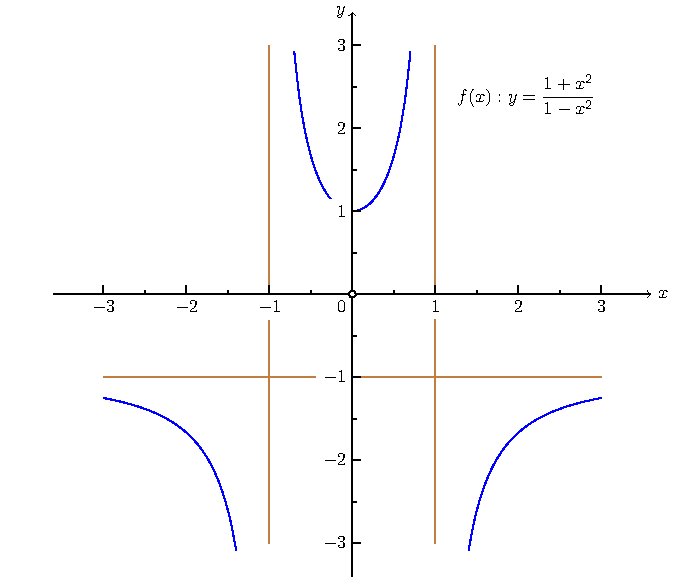
\includegraphics[width=1\linewidth]{mai_fig028.pdf}
    \captionof{figure}{Graf funkce $f(x):y=\dfrac{1+x^2}{1-x^2}$}
    \label{MAI:fig_028}
  \par}
\end{mathexam}  